\documentclass{article}

\setlength{\headsep}{0.75 in}
\setlength{\parindent}{0 in}
\setlength{\parskip}{0.1 in}

%=====================================================
% Add PACKAGES Here (You typically would not need to):
%=====================================================

\usepackage[margin=1in]{geometry}
\usepackage{amsmath,amsthm}
\usepackage{fancyhdr}
\usepackage{enumitem}
\usepackage{graphicx}
%=====================================================
% Ignore This Part (But Do NOT Delete It:)
%=====================================================

\theoremstyle{definition}
\newtheorem{problem}{Problem}
\newtheorem*{fun}{Fun with Algorithms}
\newtheorem*{challenge}{Challenge Yourself}
\def\fline{\rule{0.75\linewidth}{0.5pt}}
\newcommand{\finishline}{\vspace{-15pt}\begin{center}\fline\end{center}}
\newtheorem*{solution*}{Solution}
\newenvironment{solution}{\begin{solution*}}{{\finishline} \end{solution*}}
\newcommand{\grade}[1]{\hfill{\textbf{($\mathbf{#1}$ points)}}}
\newcommand{\thisdate}{\today}
\newcommand{\thissemester}{\textbf{Rutgers: Spring 2021}}
\newcommand{\thiscourse}{CS 440: Introduction to Artificial Intelligence} 
\newcommand{\thishomework}{Number} 
\newcommand{\thisname}{Name} 

\newcommand{\thisheading}{
   \noindent
   \begin{center}
   \framebox{
      \vbox{\vspace{2mm}
    \hbox to 6.28in { \textbf{\thiscourse \hfill \thissemester} }
       \vspace{4mm}
       \hbox to 6.28in { {\Large \hfill Project \#\thishomework \hfill} }
       \vspace{2mm}
         \hbox to 6.28in { { \hfill \thisdate \hfill} }
       \vspace{2mm}
       \hbox to 6.28in { \emph{Names: \thisname \hfill }}
      \vspace{2mm}}
      }
   \end{center}
   \bigskip
}

%=====================================================
% Some useful MACROS (you can define your own in the same exact way also)
%=====================================================


\newcommand{\ceil}[1]{{\left\lceil{#1}\right\rceil}}
\newcommand{\floor}[1]{{\left\lfloor{#1}\right\rfloor}}
\newcommand{\prob}[1]{\Pr\paren{#1}}
\newcommand{\expect}[1]{\Exp\bracket{#1}}
\newcommand{\var}[1]{\textnormal{Var}\bracket{#1}}
\newcommand{\set}[1]{\ensuremath{\left\{ #1 \right\}}}
\newcommand{\poly}{\mbox{\rm poly}}


%=====================================================
% Fill Out This Part With Your Own Information:
%=====================================================


\renewcommand{\thishomework}{2: MineSweeper} %Homework number
\renewcommand{\thisname}{Aamna Farooq (af704), Nada Elshamaa(nhe12), and Asma Makhdoom(aam355)} % Your name
 \graphicspath{ {./images/} }

\begin{document}

\thisheading



\textbf{Representation:}
	How did you represent the board in your program, and how did you represent the information / knowledge that clue cells reveal? How could you represent inferred relationships between cells? \\
\begin{solution} \hfill \\
    $Board$: \\
    Our program used a 2-D array structure to represent the board. \\
    Each cell can be accessed using Board[x][y] where x,y are the coordinates of the cell. \\
    	   
    $Knowledge$: \\
    Our program compiles any information we retain from clues into an array called Knowledge. Knowledge is an array of of equations derived from the clue cells revealed, each equation is an array of length 2 with the first index holding a set of neighbors and the second index holding the appropriate clue. \\
    We use equations to represent the relationships between cells and make inferences using those equations. Every time a clue is revealed, our program uses the clue to add an equation to knowledge and then update the existing equations using the clue that was revealed \\
    
    $Example$: 
    \begin{tabbing}
    For the \=following board:\\
    \>[1] \=[A] \=[2] \\ 
    \>[B] \>[C] \>[D] \\
    \>[E] \>[3] \>[F] \\\\
    
	We use \=the following equation system to represent the relationship between cells: \\
	\>A+B+C = 1 \\
	\>A+C+D = 2 \\
	\>E+B+C+D+F = 3\=\\
	\>\>where A=(0,1), B=(1,0), C=(1,1), D=(1,2), E=(2,0), F=(2,2) \\\\
	
	In our \=program, this is translated in our Knowledge structure as: \\
	\> [ \=[ \{ (0,1),(1,0),(1,1) \} ,1], \\
	    \>\>[ \{ (0,1),(1,1),(1,2) \} ,2], \\
	    \>\>[ \{ (2,0),(1,0),(1,1),(1,2),(2,2) \} ,3] ]
	\end{tabbing}
	Each index could be 1 or 0 depending on whether or not it is a mine.
\end{solution}

\smallskip

\textbf{Inference:}
	When you collect a new clue, how do you model / process / compute the information you gain from it?
    In other words, how do you update your current state of knowledge based on that clue? 
    Does your program deduce everything it can from a given clue before continuing? If so, how can you be sure of this, and if not, how could you consider improving it? \\
\begin{solution} \hfill \\
    \begin{tabbing}
	In our \=program, uncovering a cell can yield two results: \\
	\>a. T\=he uncovered cell is discovered to be a mine.\\
	\>\>In this case, our program updates the knowledge base by going through every equation in\\ \>\>Knowledge and for every equation, removing the uncovered index from the set of indices and\\ \>\>subtracting 1 from the total of the equation\\\\
	
	\>\> For example, if (0,1) was discovered to be a mine, \\
	\>\>the equation \{ (0,1),(1,0),(1,1) \} ,1] would be updated to \{ (1,0),(1,1) \} ,0] \\\\\\
	
	\>b. The uncovered cell is discovered to be a safe cell with a a clue.\\
	\>\>In this case, our program uses the uncovered cell's clue and its neighbors to add a new\\ \>\>equation into Knowledge. After that, our program updates the knowledge base by going through\\
	\>\>equation in Knowledge and for every equation, removing the uncovered index from the set of\\
	\>\>indices.\\\\
	
	\>\>For example, if (0,0) was discovered to be safe with a clue of 1 in the following board:\\
	\>\>[1] \=[A] \=[2] \\ 
    \>\>[B] \>[C] \>[D] \\
    \>\>[E] \>[3] \>[F] \\
    \>\>Our program create a new equation: [\{ (0,1),(1,0),(1,1) \} ,1] and adds it to Knowledge after \\ \>\>which, it goes through knowledge and for every equation where (0,0) is present, it is removed.\\\\
    
    \>In both cases, after updating Knowledge, our program runs an Advanced Inference algorithm in a\\ \>loop updating Knowledge and the grid with its inferences until no more inferences can be made using\\ \> the information we have. Therefore, it is safe to conclude that our program deduces everything it can\\ \> from Knowledge before moving on.\\
	\end{tabbing}
\end{solution}

\smallskip

\textbf{Decisions:}
	Given a current state of the board, and a state of knowledge about the board, how does your program decide which cell to search next? 
\begin{solution} \hfill \\
	We will be using an example to walk through how our program makes decision, given a user board that is completely hidden to the improved agent. 
	\begin{tabbing}
	Our program uses a queue in order to access cells. \\
	The fir\=st ever cell is picked by our algorithm in random and en-queued, and at that point one of two things \\ could happen: \\
	
	\>a. T\=he uncovered cell is discovered to be a mine, in which case our knowledge base is updated to reflect\\ \>\>that. \\
	\>b. The uncovered cell is discovered to be safe and reveals a clue, in which case our program uses the clue\\ \>\>to add an equation to the knowledge base and then updates our knowledge base. \\\\
	
	After updating the knowledge base in both cases, our program uses an advanced inference algorithm that uses\\ rref in order to make all possible inferences from the knowledge base. Our program does that by running the\\ advanced inference algorithm in a loop and updating the knowledge base with the inferences it produces, \\additionally en-queuing all of the cells inferred to be safe and marking those inferred to be mines on the board.\\ The loop runs until advanced inference can no longer return any inferences using the current knowledge base.\\\\
	
	If the queue is empty at that point, our program selects a cell at random from the covered cells in the board and\\ en-queues it\\\\
	
	Otherwise, our program de-queues and repeats all the steps mentioned above until all the cells on the board are\\ uncovered.
	\end{tabbing}
\end{solution}

\smallskip

\textbf{Performance: }
	For a reasonably-sized board and a reasonable number of mines, include a play-by-play progression to completion or loss. Are there any points where your program makes a decision that you don’t agree with?
Are there any points where your program made a decision that surprised you? 
Why was your program able to make that decision? 
\begin{solution} \hfill \\
	Performance Solution
\end{solution}

\smallskip

\textbf{Performance: }
For a fixed, reasonable size of board, plot as a function of mine density the average final score (safely identified mines / total mines) for the simple baseline algorithm and your algorithm for comparison. This will require solving multiple random boards at a given density of mines to get good average score results.
Does the graph make sense / agree with your intuition? When does minesweeper become ‘hard’?
When does your algorithm beat the simple algorithm, and when is the simple algorithm better? Why?
How frequently is your algorithm able to work out things that the basic agent cannot?
\begin{solution} \hfill \\

    \begin{figure}[h]
	\centering
	\IfFileExists{images/performance_plot.png}{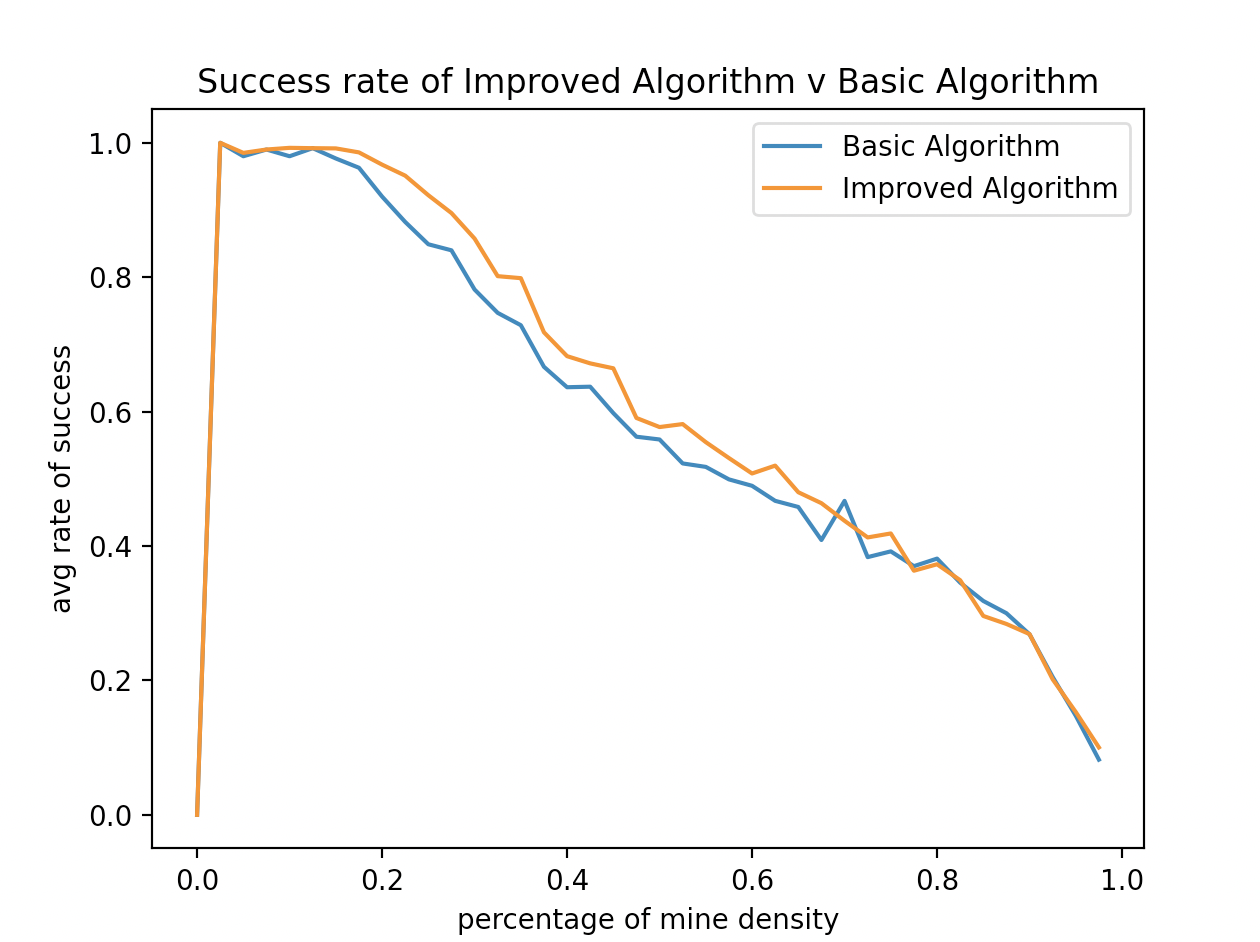
\includegraphics[width=0.7\textwidth]{images/performance_plot.png}}{No Figure Yet}
% 	\includegraphics[width=12cm]{dim100,50avg,step01}
	\caption{Plot of a function of mine density and the average final score (safely identified mines / total mines) for the simple baseline algorithm and our improved algorithm for comparison using a dimension of 20 and average of 10 random boards per given mine density}
	\end{figure}

\end{solution}

\smallskip

\textbf{Efficiency: }
What are some of the space or time constraints you run into in implementing this program? 
Are these problem specific constraints, or implementation specific constraints? 
In the case of implementation constraints, what could you improve on?
\begin{solution} \hfill \\
   Efficiency Solution
\end{solution}

\smallskip

\textbf{Global Information: }
	Suppose you were told in advance how many mines are on the board. Include this in your knowledge base. How did you model this? Regenerate the plot of mine density vs average final score with this extra information, and analyze the results.
\begin{solution} \hfill \\
	Global Information Solution
\end{solution}

\smallskip

\textbf{Better Decisions: }
	In both the basic and improved agent, when nothing more could be inferred, the agent selects a covered cell at random. Build a better selection mechanism. How can you justify it? Regenerate the plot of mine density vs average final score with improved cell selection, and analyze the results.
\begin{solution} \hfill \\
     Better Decisions Solution
\end{solution}

\textbf{Work Distribution}
\\
The work is our own and not copied or taken from any other students. 
\\\\
To work on this project we would meet up over video calls daily and discuss problems and our solutions. One person would then screen share and code while the others would contribute and also assist in coding using the request remote control feature in zoom. We would alternate in screen sharing and upload to git for version control. 
\\\\
The report was done similarly. We each took on a plot and a question to complete on our own. We then met to complete the rest as a group over video call. 
\\
$Asma$ $Makhdoom:$ Problem 2
\\
$Aamna$ $Farooq:$ Problem 3
\\
$Nada$ $Elshamaa:$ Problem 4 and Problem 6
\\
\smallskip

\end{document}